\documentclass{CST_CryptoIntro}
\usepackage{indentfirst}
% ===== 封面配置 =====
\reportCourse{密码分析学实验报告}
\reportLogo{figures/logo_sduWithText.jpg}
\reportName{邱泽辉、江李阳、王健一}
\reportID{202400460046、202400460042、202400460037}
\reportMajor{密码科学与技术}

% ===== 页眉配置 =====
\headerLeft{密码分析学}
\headerRight{第一次实验实验报告}

\begin{document}

% ===== 封面 =====
\maketitle
\thispagestyle{fancy}
\newpage

% ===== 目录 =====
\tableofcontents
\newpage

% ================================================================
% 正文内容
% ================================================================
\section{实验目的}

本实验围绕 Enigma 密码机的结构、加密过程和密钥空间展开。通过编程实现给定参数下的 Enigma 加密，理解接线板、转子和反射器在密码变换中的作用；在此基础上分析转子排列、转子起始位置和接线板设置所形成的密钥空间，并结合实际加密速度判断直接穷举攻击的可行性。

\subsection{组员分工}
\begin{itemize}
    \item 邱泽辉（202400460046）：任务一、任务二的实现以及任务二的撰写。
    \item 江李阳（202400460042）：任务一、任务三的实现以及报告主体的撰写。
    \item 王健一（202400460037）：任务二的实现以及报告的补充、修改与整合。
\end{itemize}
% 实验环境
\input{content/1environment}

%实验原理
\input{content/2principle}

%实验内容

\section{任务一}
\subsection{Enigma密码机程序编写}
按照实验指导书的配置设置 Enigma 机的加密代码，本部分在参考程序的基础上进行整理和修改，主要完成以下配置：
\begin{itemize}
    \item 使用 5 条连线的接线板 $S=[AV\ BS\ CG\ MN\ OX]$ 设置密钥 $K_1$；
    \item 使用实验指导书给出的三个转子，按照快速、中速、慢速的顺序设置为 $I$、$II$、$III$，并将起始位置设置为 $K_2=(8,9,10)$；
    \item 设置反射器 $T$。反射器是实验给定的固定部件，不作为本实验中需要恢复的密钥部分。
\end{itemize}

\subsection{测试Enigma密码机}
使用编写完成的 Enigma 机程序加密给定明文 \texttt{WETTER}，输出密文为 \texttt{TWNVCX}，运行结果如下图所示：
\begin{figure}[H]
    \centering
    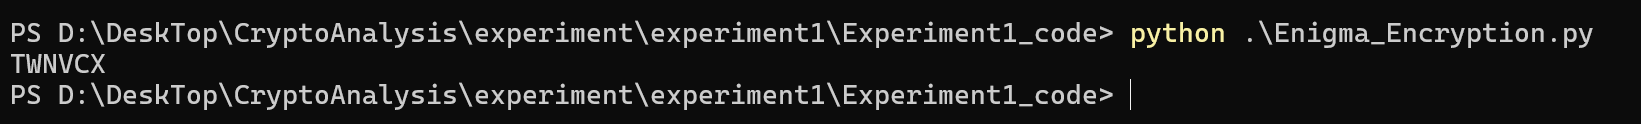
\includegraphics[width = 1\textwidth]{figures/task1_enigma_encryption.png}
    \caption{Enigma机加密测试明文}
\end{figure}
由输出结果可知，程序能够按照实验指导书给定的接线板、转子、反射器和起始位置完成明文加密。

\input{content/task2/task2.tex}
\section{任务三}
任务三要求在从 4 个转子中选择 3 个后进行加密。为便于说明，先给出三个转子固定、但转子顺序未知时的密钥空间。

三个固定转子的排列有 $3!$ 种，每个转子的起始位置有 26 种可能，因此

\begin{equation*}
    N_{K_2}=3!\times26^3=105,456\approx2^{16.69}.
\end{equation*}

按照实验指导书和参考程序中的限制，接线板最多有 6 条接线。严格计算所有允许的接线数量时，

\begin{equation*}
    N_{K_1}=\sum_{l=0}^{6}\frac{26!}{(26-2l)!2^l l!}
    =105,578,918,576\approx2^{36.62}.
\end{equation*}

因此，三个转子固定但顺序未知时的完整密钥空间为

\begin{equation*}
    N=N_{K_1}N_{K_2}
    =11,133,930,437,350,656
    \approx2^{53.31}.
\end{equation*}

若按照最大接线数 $l=6$ 的最大项进行数量级估计，则 $N_{K_1}(6)\approx2^{36.55}$，相应的总密钥空间约为 $2^{53.23}$，同样可以近似记为 $2^{53}$。

当从 4 个转子中选择 3 个并安排顺序时，转子部分的排列数量变为

\begin{equation*}
    N_{K_2}'=P_4^3\times26^3
    =24\times26^3
    =421,824\approx2^{18.69}.
\end{equation*}

接线板的可能数量不变，因此任务三的完整密钥空间为

\begin{equation*}
    N'=N_{K_1}N_{K_2}'
    =44,535,721,749,402,624
    \approx2^{55.31}.
\end{equation*}

若采用 $l=6$ 最大项估算，则

\begin{equation*}
    N'_{l=6}=N_{K_1}(6)N_{K_2}'
    =42,347,667,057,696,000
    \approx2^{55.23}.
\end{equation*}

因此任务三理论上需要猜测约 $2^{55}$ 个完整密钥。

对任务一中的 Enigma 加密程序进行性能测试，采用 1000 条长度为 6 的随机明文并统计加密时间，测试结果如下：
\begin{figure}[H]
    \centering
    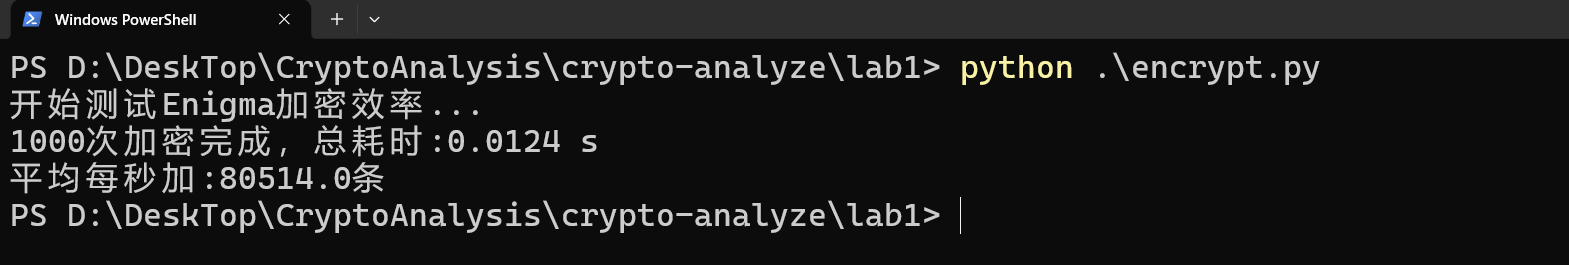
\includegraphics[width = 1\textwidth]{figures/task3_encrypt_efficiency.png}
    \caption{测试Enigma加密效率}
\end{figure}
测试结果显示每秒约可完成 80514 次加密\footnote{测试明文长度均为 6，随机明文在计时前生成；测试循环中复用同一台 Enigma 机器，因此测量的是连续加密吞吐量。}。若采用严格的“不超过 6 条接线”密钥空间进行估计，则直接穷举所需时间为

\begin{equation*}
    T=\frac{N'}{80514}
    \approx5.53\times10^{11}\text{ s}
    \approx9.22\times10^9\text{ min}
    \approx6.40\times10^6\text{ d}
    \approx1.75\times10^4\text{ 年}.
\end{equation*}

若按 $l=6$ 最大项近似，则所需时间约为 $5.26\times10^{11}$ s，即约 $1.67\times10^4$ 年。两种计算结果均表明，在个人计算机上直接穷举任务三的完整密钥空间完全不可行。


\section{实验总结}
\indent 这次实验围绕 Enigma 密码机的加密实现、密钥恢复和密钥空间分析展开。通过模拟接线板、扰频器与反射器及其反向过程，
我们进一步理解了 Enigma 的加密结构以及转子状态变化对加密结果的影响。在给定参数下，程序将明文 WETTER 加密为 TWNVCX，
与预期结果一致，验证了该配置下加密流程的正确性。

在密钥恢复部分，我们在中速和慢速转子不转动的假设下，利用已知明密文中的特殊的Crib环路关系建立约束，
将转子设置的搜索与接线板映射的恢复分开处理，对密钥空间进行分割。通过多个环路筛选候选，再利用完整明密文关系扩展映射、排除矛盾，最终
得到转子初始位置 \((3,14,7)\) 及部分接线板映射。这一过程使我们认识到，密码分析可以利用密码结构与已知信息对搜索范围进行分割，
而较大的理论密钥空间并不意味着能够抵抗所有分析方法。

在密钥空间与性能分析部分，当从四个转子中选择三个并允许接线板最多使用六条接线时，
总密钥空间约为 \(2^{55.31}\)。根据实验测得的连续加密吞吐量进行粗略估算，遍历完整密钥空间需要约 \(1.75\times10^4\) 年，说明在本实验的实现与现有的硬件条件下，
在个人计算机上直接穷举任务三的完整密钥空间完全不可行。


通过本次实验，我们加深了对于 Enigma 密码机各个部件及其作用的理解，也体会到了程序实现、结果验证与复杂度分析需要相互配合。
后续可通过增加已知明密文补全尚未确定的接线板映射，并在更完整的转子转动条件下检验攻击方法的适用性。
\clearpage
\appendix
\section{实验代码}

本附录列出本次实验中使用的 Enigma 加密及性能测试程序。

\subsection{Enigma 加密及性能测试程序}
\lstinputlisting[caption={encrypt.py}]{../encrypt.py}

\section{实验报告完整地址}
实验完整代码、实验报告 \LaTeX{} 源代码见仓库：
\url{https://github.com/infinitepwn/crypto-analyze.git}




% \section{参考资料}
% \begin{enumerate}
%     \item 《密码分析学实验一》实验指导书。
%     \item 课程课件《密码分析学概述》和《恩尼格玛密码机的破解》。
%     \item 实验目录中的 Enigma 参考程序，并在报告任务一中对相应参考内容作出说明。
% \end{enumerate}





% \section{算法测试效率}

% \subsection{正常使用测试}

% 测试结果如下表所示:

% \begin{table}[H]
%     \centering
%     \caption{正常流程各阶段性能数据}
%     \begin{tabular}{@{}llcc@{}}
%         \toprule
%         阶段 & 描述 & 耗时 & 占比 \\
%         \midrule
%         Step 0   & 证书获取与连接       & $117.00$\,ms  & 99.5\% \\
%         Phase 1--2 & 密钥协商          & $17.47$\,ms  & 74.6\% \\
%         Phase 3   & 加密航班查询        & $3.44$\,ms   & 14.7\% \\
%         \midrule
%         \textbf{总计} & —              & $\mathbf{23.41}$\,\textbf{ms} & — \\
%         \bottomrule
%     \end{tabular}
% \end{table}

% \subsection{关键代码}

% 代码示例 (\texttt{ca/certificate\_authority.py}):

% \begin{lstlisting}[caption={ca/certificate\_authority.py — issue\_agent() \& verify\_certificate()}]
% def issue_agent(self, agent_id, permissions):
%     # 1. 生成 Agent 的 Ed25519 密钥对
%     signing_private = generate_keypair()
%     cert_body = {
%         "agent_id": agent_id,
%         "public_key": b64e(signing_private.public_bytes_raw()),
%         "permissions": permissions,
%     }
%     # 2. CA 使用 Ed25519 私钥对证书体签名
%     certificate = {
%         "body": cert_body,
%         "ca_signature": sign(self.private_key, cert_body),
%     }
%     return certificate

% def verify_certificate(self, certificate):
%     body = certificate["body"]
%     # 验证 CA 签名
%     verify(self.public_key, certificate["ca_signature"], body)
%     return body["agent_id"]
% \end{lstlisting}

% \section{实验结果分析与总结}

% 本实验完整覆盖了证书颁发、密钥协商、授权管理等全流程，协议在各层面均表现出有效的防护能力。

% \appendix
% \section{附录}

% 项目完整代码地址: \url{https://github.com/example/crypto-intro.git}

\end{document}
